\documentclass[10pt,twocolumn]{article}

\usepackage{amsfonts}
\usepackage{amsmath}
\usepackage{authorship}
\usepackage{graphicx}
\usepackage{ieee}
\usepackage{mailto}
\usepackage{nicefrac}
\usepackage{subfigure}
\usepackage{url}
\usepackage{xspace}

\usepackage[bookmarks, pdftitle={Public Deployment of Cooperative Bug
  Isolation}, pdfauthor={Ben Liblit, Mayur Naik, Alice X. Zheng, Alex
  Aiken, and Michael I. Jordan}, pdfpagemode=UseOutlines]{hyperref}

\ifthenelse{\isundefined{\pdfoutput}}{}{\usepackage{thumbpdf}}

\newcommand{\evolution}{Evolution\xspace}
\newcommand{\gaim}{Gaim\xspace}
\newcommand{\gimp}{The GIMP\xspace}
\newcommand{\gnumeric}{Gnumeric\xspace}
\newcommand{\nautilus}{Nautilus\xspace}
\newcommand{\rhythmbox}{Rhythmbox\xspace}

\newcommand{\header}[1]{\multicolumn{1}{c}{\textbf{#1}}}

\newcommand{\termdef}[1]{\emph{#1}}

\pagestyle{empty}

\begin{document}

\title{Public Deployment of Cooperative Bug Isolation
  %%
  \thanks{This research was supported in part by NASA Grant No.\ 
    NAG2-1210; NSF Grant Nos.\ EIA-9802069, CCR-0085949, ACI-9619020,
    and IIS-9988642; DOE Prime Contract No.\ W-7405-ENG-48 through
    Memorandum Agreement No.\ B504962 with LLNL; and DARPA ARO-MURI
    ACCLIMATE DAAD-19-02-1-0383.  The information presented here does
    not necessarily reflect the position or the policy of the
    Government and no official endorsement should be inferred.}}

\author{%
  Ben Liblit \eecs \\ \aumail{liblit@cs.berkeley.edu} \and
  Mayur Naik \stan \\ \aumail{mhn@cs.stanford.edu} \and
  Alice X.\ Zheng \eecs \\ \aumail{alicez@cs.berkeley.edu} \and
  Alex Aiken \stan \\ \aumail{aiken@cs.stanford.edu} \and
  Michael I.\ Jordan \both \\ \aumail{jordan@cs.berkeley.edu}
  %%
  \aupar
  %%
  \eecs Department of Electrical \\ Engineering and Computer Science \\
  \stat Department of Statistics \\
  University of California, Berkeley \\
  Berkeley, CA 94720-1776
  %%
  \and
  %%
  \stan Computer Science Department \\
  353 Serra Mall \\
  Stanford University \\
  Stanford CA 94305-9025
}

\maketitle

\thispagestyle{empty}

\begin{abstract}
  As part of our work on Cooperative Bug Isolation (\termdef{CBI}) we
  have undertaken to instrument and distribute binaries for a number
  of large open source projects.  This public deployment is an
  important step toward a large experiment involving (we hope)
  hundreds or thousands of users that will measure the effectiveness
  of CBI\@.  This paper describes several of the significant
  engineering issues that arise in instrumenting the source code of
  realistic applications.
\end{abstract}

\section{Introduction}

Cooperative Bug Isolation (\termdef{CBI}) seeks to leverage the huge
amount of computation done by the end users of software.  By gathering
a little bit of information from every run of a program performed by
its user community, we should be able to make inferences automatically
about the causes of bugs experienced in the field.

Our approach to CBI is based upon compile-time instrumentation of the
program's source code.  We insert instrumentation to
test a large number of predicates on program values during
execution and to count how many times each predicate is observed to be
true or false.  On termination of the program the list of predicate
counters is uploaded to a central server together with a record of
whether the program terminated successfully or not.  Subsequent
statistical analysis of which predicates are correlated with program
failure can then indicate to engineers which values and what parts of
the program are the sources of crashes; in at least some cases even
the exact line of code that is at fault can be identified
\cite{PLDI`03*141,Liblit:2003:SUEBI,Zheng:2003:SDSP}.

We believe that CBI and related research efforts have great potential
to make software development more responsive and efficient by giving
developers accurate data about how software is actually used in
deployment.  However, testing this idea requires significant
experimentation with real, and preferably large, user communities
using real applications.

This paper reports on our experience in preparing for just such an
experiment.  We have instrumented a number of large open source
applications, listed in \autoref{apps}, with a total of about 1.8
million lines of code. We have made these instrumented programs
available to the public and are in the process of collecting feedback
reports.  As a result, we have demonstrated a complete CBI system and
feel comfortable in claiming that our approach is technically
feasible; while aspects of our system could certainly be improved, at
this point all components are good enough to support the deployment of
realistic instrumented applications and the collection of feedback
reports from a large user community.

The design of a CBI system involves interesting challenges, both
technical and social.  In this paper, we focus on the solutions to
technical problems most likely to be useful to the designers of
similar systems and experiments: dealing with existing native
compilers, shared libraries, plugins, and threads.  We also briefly
discuss how users interact with our system, as well as give some
static and dynamic measures of the applications we instrument.

\begin{table*}
  \centering
  \begin{tabular}{lrcccc}
    \header{Application} & \header{Lines of Code} & \header{Shared Libraries} & \header{Plugins} & \header{Threads} \\\hline
    \evolution  & 460,912 & \checkmark & \checkmark & \checkmark \\
    \gaim & 160,435 & & \checkmark & \\
    \gimp & 650,660 & \checkmark & \checkmark & \\
    \gnumeric & 319,137 & & \checkmark & \\
    \nautilus & 124,679 & \checkmark & \checkmark & \checkmark \\
    \rhythmbox  &  56,442 & \checkmark & &
  \end{tabular}
  \caption{Instrumented applications}
  \label{apps}
\end{table*}

\section{Native Compiler Integration}

The system as a whole looks and behaves like GCC with a few extra
command line flags.  No manual annotation of source code is required,
and all existing configuration scripts and makefiles work
transparently.  This lets us instrument 1.8 million lines of open
source code and keep up with new releases with very short turnaround.
Simply changing an environment variable (\texttt{\$CC}) builds an
application with our instrumenting compiler instead of the standard
one.

The meat of instrumentation happens as a source to source
transformation after the preprocessor and before the real C compiler.
However, we actually need to affect all stages of compilation:

\begin{description}
\item[before preprocessing (\texttt{cpp0}):] Pull in extra headers to
  declare or define various constructs used by instrumented code.  For
  fixed content such as this it is easier to use fixed headers rather
  than synthesizing the needed constructs programmatically within the
  instrumentor.
  
\item[before compilation (\texttt{cc1}):] Inject sampled
  instrumentation as a source-to-source transformation.  Emit
  additional static site information into temporary files for use in
  next step.
  
\item[after assembly (\texttt{asm}):] Fuse extra static site
  information from temporary files into the assembled object file.
  
\item[before linking (\texttt{ld}):] Pull in extra libraries
  containing common runtime support code and data used by instrumented
  programs.
\end{description}

We use GCC's \texttt{-B \textit{<path>}} flag to specify an alternate
directory in which to find the compiler stages.  Custom scripts in
that directory named \texttt{cc1} and \texttt{asm} do the extra
``before compilation'' and ``after assembly'' work and invoke the
corresponding native compiler stages as appropriate.

We also use GCC's \texttt{-specs=\textit{<file>}} flag to augment (not
replace) the standard option specs file with one of our own.  An
\termdef{option specs file}, or simply ``specfile,'' determines how
GCC parses its command line arguments.  We can add flags of our own,
request temporary file names, and so on.  A specfile is essentially a
tiny domain-specific language for tweaking the command lines used for
the various compiler stages.  Using this facility we are able to take
care of our ``before preprocessing'' and ``before linking'' needs by
augmenting the \texttt{cpp0} and \texttt{ld} command lines without
actually replacing those stages with custom scripts of our own.

\subsection{Static Site Information}

While the main ``before compilation'' task is to inject
instrumentation code, that this phase also produces static reference
information about each instrumentation site.  This includes each
site's source file name, line number, host function, control flow
graph node, and other information specific to the instrumentation
scheme being used.  When decoding feedback reports, this information
is used to tie predicate counts back to source level features
understood by the programmer.  Our experience is that maintaining this
information external to the corresponding object file is brittle, as
existing application build scripts often move or rename object files
during the build process.  Therefore, we fuse the static site
information into the assembled object file by storing it in several
custom ELF sections.

When the linker combines several object files, it pads each unknown
section out to some fixed modulus and then concatenates all same-named
sections in link order.  We represent our static site information in a
way that remains valid under null-byte injection and concatenation.
Thus each instrumented executable, shared library, or plugin is self
describing, with complete static information for all of its own
instrumentation sites.  Our extra sections are flagged as debug
information, which means that they will be stripped out along with
other debugging information during post-build packaging.  We retain a
copy locally to assist in report decoding, but end users do not need
to download and store this extra information on their own machines.

\section{Libraries and Plugins}

Post-run reporting would be easy for an application that consisted of
a single object file.  We would simply write out the predicate
counters in the order in which they appear in that file, and that list
would constitute a complete report.

However, as can be seen in \autoref{apps}, most applications involve
multiple object files in the form of shared libraries, plugins, or
both.  Note that this table counts only those shared libraries and
plugins that are part of the source code of the application;
additionally, there generally will be other shared
libraries and plugins that are resident only on the end user's
machine.  Thus, the running environment is a mix of code that has
been instrumented by CBI and code that we have never seen before.
Shared libraries are also interesting because they may be used by
other applications that we have not instrumented.  Thus, not only must
instrumented applications cope with uninstrumented code, but
instrumented code must cope with finding itself in an
uninstrumented application.

An orthogonal set of problems arises from static linking and dynamic
loading.  Our system does not have control over the linker and
cannot assume that object files appear in any particular order.
Plugins may be loaded late and unloaded at any time.  If an
instrumented plugin is about to be unloaded, we must capture its part
of the feedback report immediately, because once it is unloaded its
global predicate counters vanish from the address space and can no
longer be accessed.

Our solution to all of these problems is to make each object file
self-managing, with some initialization code that runs when it is
loaded, and finalization code that runs when it is unloaded.  For
objects which are part of the main application binary, the
initialization code runs early in program execution, before
\texttt{main()}.  The finalization code runs after \texttt{main()}
returns or after \texttt{exit()} is called.  Shared libraries are
similar.  For plugins, the initialization code runs within
\texttt{dlopen()} after the plugin has been mapped into memory.
Plugin finalization code runs within \texttt{dlclose()} just before
the plugin is removed from memory.  Each object file also maintains
its own instrumentation state; in particular, each object file maintains
its own predicate counters.

There is one situation in which we need global knowledge of the loaded
object files.  Finalization code does not run after a crash.  Thus if
the program receives a fatal signal, we must immediately gather the
predicate counters from each loaded object file for the feedback
report.  We maintain a doubly-linked list of loaded object files, and
the initialization/finalization code for each object file adds/removes
that file from this list.  Thus at any moment in time the application
has a central registry of all instrumented, currently loaded object
files.

We have also given some attention to the fact that this global
registry could itself be corrupted by a buggy program.  We maintain a
global count of the expected size of the global registry.  When
walking the list in a signal handler, we use the counter to decide
when to stop even if we have not reached the end of the list data
structure.  This prevents an infinite loop if a memory error in the
application introduces a cycle into the doubly-linked list.  The
global registry can be damaged in other ways by a misbehaving program,
of course, but avoiding cycles is the most important case to handle.

The complications in checking for a corrupted global registry are just
an example of the general problem that it is not possible to
completely isolate program instrumentation from the program itself in
unsafe languages such as C and C++.  As a result it is necessary to
sanity check feedback reports at the central server and discard any
that are ill-formed.  In practice we do receive ill-formed reports,
but the number is only a tiny fraction of all reports.

\section{Threads}

Our CBI system maintains three kinds of global data that need special
attention in multi-threaded applications.  In each case thread-safety
can hurt performance, so we only take this extra care if in fact the
application is multi-threaded (e.g.\ if the compiler's command line
contains the GCC \texttt{-pthread} flag).

A key feature of our CBI system is that performance can be improved by
sampling the instrumentation code, which is implemented by frequently
skipping over some instrumentation and instead executing a ``fast
path'' with no instrumentation at all.  We use a \termdef{global
  countdown} to determine how many instrumentation sites to skip
before testing one predicate and recording its result.  The countdown
is chosen randomly from a geometric distribution with a mean that is
the desired sampling rate.  (This is equivalent to, but much more
efficient than, tossing a coin at each instrumentation site to decide
whether to take a sample.)  In a multi-threaded system, the global
variable holding this next-sample countdown would be a source of high
contention among threads.

The simple solution to this problem is to give each thread its own,
independent countdown variable.  This is equivalent to giving each
thread its own coin to toss.  The behavior of the system with
per-thread countdowns is indistinguishable from having a single global
countdown, and in addition we avoid all locking.

Enacting this plan requires compiler support.  We use the
\texttt{\_\_thread} storage qualifier to declare thread-specific
storage.  This is a GCC extension and also requires support from the
POSIX threading runtime, C library, and runtime loader.  We also must
alter thread creation so we can initialize the new thread's global
state.  We use the \texttt{--wrap} flag provided by the GNU linker to
replace \texttt{pthread\_create()} with our augmented version.

The second class of data that requires special handling in
multi-threaded applications is the predicate counters.  Recall that
the predicate counters keep track of how often a particular predicate
at a particular line of code is observed to be true or false.  For
efficiency we use low sampling rates, such as once every hundred times
(on average, randomized) that the line of code associated with the
predicate is executed.  Therefore predicates are tested rarely and any
individual counter is accessed rarely even by a single thread.
Therefore, we maintain only one copy of each predicate counter, shared
by all threads.  The critical operation on these counters, an
increment by one, is so basic that every CPU architecture has some way
of doing this atomically without resorting to heavyweight locking.

Finally, the third class of data that must be protected from
concurrent access includes the global registry of compilation units
and the report file.  Because these structures are accessed very
rarely, we guarantee exclusive access by guarding each with its own
mutual exclusion lock.


\section{User Interaction}

When a user launches an instrumented application, he does not run the
instrumented binary directly.  Instead, we install a wrapper script in
the expected location (e.g. \texttt{/usr/bin}) and put the
instrumented binary elsewhere.  The wrapper script has several
responsibilities: it performs all user interaction that goes beyond
what the underlying application would normally do, and it collects the
raw feedback report from the instrumented application, packages it for
transit, and sends it to the report collection server along with other
information such as program outcome.  In this way we avoid adding GUI
infrastructure and encrypted networking support to the applications
themselves.  Also, the script can be in a different language, Python,
which has excellent library support for both networking and desktop
interaction.

\begin{figure}
  \centering
  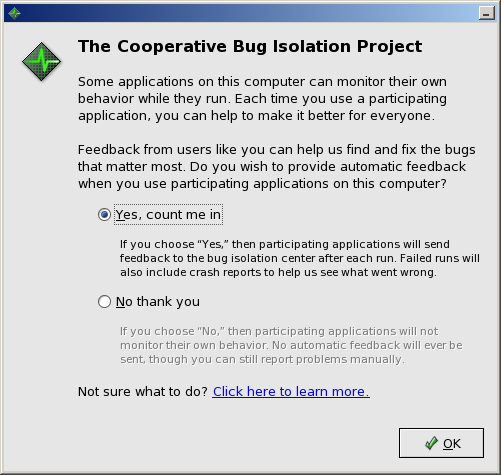
\includegraphics[width=\columnwidth]{first-time}
  \caption{First-time opt-in dialog box}
  \label{first-time}
\end{figure}

When the wrapper script starts up, it checks whether the user has run
an instrumented version of this application before.  If not, it
presents the first-time opt-in dialog box shown in
\autoref{first-time}. The dialog box briefly describes the goals of
the project and the consequences of participating or not, and lets the
user decide what to do.  The logo icon and highlighting of the yes/no
explanatory text change to reflect user's current choice.  A hyperlink
button links to the project web site for more information
\cite{Liblit:CBIP}.  This dialog box is initially presented in the
background, and the real application launched without waiting for a
reply.  On this first run, the application reports no data. Once the
user has selected yes or no, that preference is remembered and the
first-time opt-in dialog box is not shown on subsequent runs, though
it is possible to change the preference later using a distinct sampler
control panel.

Also in the background, the wrapper posts a small status icon in
the desktop status bar notification area.  This icon provides a
visual reminder that an instrumented application is currently
running. It provides a simple pop-up menu with a toggle to globally
disable or enable sampling.  The status icon changes depending on
whether sampling is enabled or disabled globally, and remains present
as long as at least one instrumented application is running.  A second
menu item launches the sampler control panel which allows for
more detailed customization of data collection preferences.

The opt-in dialog box, status icon, and control panel work together to
keep the user fully informed and fully in control.  Additional
configuration management hooks let system administrators change both
defaults as well as mandatory, locked-down settings.  These settings
can include the sampling density, the address of the report collection
server, and whether reporting is enabled for all or selected
applications.  Tracking of user behavior is a delicate matter, so
users and their system administrators must be able to adapt the system
to local needs and concerns.

\begin{table}
  \centering
  \begin{tabular}{lrr}
    \header{Application} & \header{Min} & \header{Max} \\ \hline
    \evolution & 830 & 39,863  \\
    \gaim & 1,786 & 18,772  \\
    \gimp & 15,617 & 26,304  \\
    \gnumeric & 6,661 & 15,876  \\
    \nautilus & 3,252 & 10,638  \\
    \rhythmbox & 897 & 5,823 
  \end{tabular}
  \caption{Feedback report sizes in bytes}
  \label{report-sizes}
\end{table}

Because the wrapper script launches the instrumented binary as a
subprocess, it can also check that subprocess's exit status (either a
result code or a fatal signal), which is included in the report
uploaded to our feedback collection server.
The wrapper script compresses the raw feedback report for transit
using \texttt{gzip}-compatible compression.  This is a huge benefit, as reports
are mostly zeros and compress very well.  The average compression
of the reports we have received is 96\%; \autoref{report-sizes} shows
the range of report sizes we have received by application.  
The largest reports are less than 40K bytes, which can be uploaded
over even a slow modem connection in seconds.

Before submitting a report, the wrapper checks once more whether
sampling is enabled both globally and for this application.  If the
user changed his mind after program launch, this gives a second chance
to quash an unwanted feedback report before it reaches the collection
server.

A report is submitted using an HTTP POST request across an encrypted SSL
connection.  Each HTTP request can also have a response from the server.
Ordinarily the collection server does not give any response beyond a
success code.  However, if the server does give a response, the
wrapper script receives it and presents it to the user as an HTML
page.  This feature might be used, for example, if a critical security
issue were found requiring immediate upgrades.  

The HTTP reply can also include a few special reply headers which
update the local sampling configuration on the client.  We have the
ability to promote a different destination URL for future reports,
which may be useful if we need to relocate the collection server.  We
can change the sampling density from its default of
$\nicefrac{1}{100}$, which may be useful if performance problems
arise.  We can also issue a ``poison pill'' which turns off sampling
for future runs of the application.  This is intended as a shutoff
should the Cooperative Bug Isolation project be discontinued at some
future date (a feature we learned would be useful from the prior
experience of Elbaum and Hardojo \cite{Elbaum:2003:DISATA}), and it
might also be used to suppress future reports from individual
misbehaving users.  So far we have not needed any of these facilities.

\section{Status of the Public Deployment}

We conclude with some discussion of our experience thus far with our public
deployment of the applications listed earlier.

One concern is that our approach adds a great deal of new code
to an application; in fact, binaries will often be at least twice as
large as the original, uninstrumented program.  However, the growth in
disk footprint is considerably smaller if one considers the entire
package that comes with a typical large application, and in fact the
executable code is often a relatively small percentage of the total
distribution.  For the applications we have instrumented, downloaded
packages are between 13\% and 49\% larger and the installed footprint
on disk grows between 13\% and 71\%.  The actual application binaries
are between 74\% and 304\% larger than in the original distribution.
Thus far we have received no complaints about package sizes, either
downloaded or as expanded onto disk.

Another potential issue is application performance, but thus far we
have received no complaints about the performance of any of our
instrumented applications.  We use \nicefrac{1}{100} sampling, which
apparently is sparse enough; we probably could have sampled even more
densely for these interactive applications which spend most of their
time waiting for the user to do something.  Note however that 
these applications do have CPU-intensive phases, such as when
\rhythmbox is loading up a library with thousands of music files or
when \gnumeric is recalculating a very large spreadsheet.

\begin{table}
  \centering
  \begin{tabular}{lrrrr@{~(}r@{\%)}}
    \header{Application} & \header{Total} & \header{Good} & \header{Error} & \multicolumn{2}{c}{\textbf{Crash}} \\ \hline
    \evolution & 916 & 838 & 55 & 23 & 3 \\
    \gaim & 495 & 417 & 62 & 16 & 4 \\
    \gimp & 109 & 107 & 2 & 0 & 0 \\
    \gnumeric & 261 & 242 & 2 & 17 & 7 \\
    \nautilus & 747 & 642 & 96 & 9 & 1 \\
    \rhythmbox & 869 & 728 & 39 & 102 & 14
  \end{tabular}
  \caption{Number of reports received to date}
  \label{reports-per-app}
\end{table}

\autoref{reports-per-app} summarizes the current state of the data for
each of our instrumented applications.  The \emph{total} number of
valid feedback reports received so far is broken out into \emph{good}
runs, runs that exited with a non-zero \emph{error} status, and runs
that ended in a \emph{crash} due to a fatal signal.  Note the large
variation in crash rates, from 0\% (\gimp) to 14\% (\rhythmbox).

There is both good news and bad news in these figures.  The bad news
is that we have not yet received enough reports to carry out
statistically significant analysis of the results, based on our
previous experience with studies done ``in the lab'' running
applications on synthetic data to simulate a large user community.
With $\nicefrac{1}{100}$ sampling we need between ten and twenty
thousand runs with our current methods to achieve accurate analysis of
the results, which is more than ten times the number of reports we
have received to date for any of these applications.\footnote{We began
  collecting data from the public in October, 2003.}  Our situation
here reflects an inherent aspect of CBI and similar approaches, which
is that these methods work well only beyond a certain minimum scale.

The good news is that these applications do crash,
indicating to us that there is potential to improve the state
of the software given enough users participating in CBI\@.  In addition,
we have enough data to demonstrate that the complete system works, from
instrumenting code through gathering of reports, and we continue to
receive new feedback reports daily.  We are only at the beginning of this
experiment and have not yet invested much effort in attracting users. 
The next step in our experiment will be
to find ways to recruit enough users to test the advantages of CBI
for large user communities of complex applications.

\bibliography{personal,pldi03,ramss}

\end{document}

%% LocalWords:  CBI plugins lrcccc specfile plugin pthread Elbaum
%% LocalWords:  Hardojo lrr lrrrr pldi ramss
